\documentclass[a4paper,12pt]{article}

% --- Packages ---
\usepackage[utf8]{inputenc}
\usepackage[T1]{fontenc}
\usepackage[margin=1in]{geometry}
\usepackage{amsmath, amssymb, amsthm, mathtools}
\usepackage{physics}      % For \bra, \ket, \abs, \norm, etc.
\usepackage{graphicx}
\usepackage{cancel}       % For crossing out terms
\usepackage{xcolor}       % For colors
\usepackage{fancyhdr}     % For headers/footers
\usepackage{hyperref}     % For clickable links
\usepackage{booktabs}     % For professional tables
\usepackage{array}        % For table column formatting

% --- TikZ Setup & Libraries ---
\usepackage{tikz}
\usetikzlibrary{decorations.markings, decorations.pathmorphing, arrows.meta, calc, shapes.misc, patterns}

% --- Custom TikZ Styles ---
\tikzset{
    pole/.style={cross out, draw=red, very thick, minimum size=4pt, inner sep=0pt, outer sep=0pt},
    branchcut/.style={decorate, decoration={snake, amplitude=1pt, segment length=4pt}, draw=blue!50!black, thick},
    contour/.style={thick, decoration={markings, mark=at position 0.55 with {\arrow{>}}}, postaction={decorate}, draw=black},
    region/.style={fill=blue!5, opacity=0.8}
}

% --- TColorBox Setup (Textbook Style) ---
\usepackage[most]{tcolorbox}

% 1. Definition/Formula Box (Blue Theme)
\newtcolorbox{keyconcept}[1][]{%
    enhanced,
    colback=blue!5!white,
    colframe=blue!65!black,
    fonttitle=\bfseries,
    title={#1},
    attach boxed title to top left={yshift=-2mm, xshift=2mm},
    boxed title style={colback=blue!65!black},
    sharp corners=downhill,
    arc=3mm,
    top=4mm,
    bottom=2mm,
    before skip=1em,
    after skip=1em
}

% 2. Example Box (Gray/Clean Theme)
\newtcolorbox[auto counter, number within=section]{examplebox}[1][]{%
    enhanced,
    breakable,
    colback=white,
    colframe=gray!80!black,
    fonttitle=\bfseries,
    title={Example~\thetcbcounter: #1},
    coltitle=white,
    attach boxed title to top left={yshift*=-\tcboxedtitleheight/2, xshift=5mm},
    boxed title style={colback=gray!80!black},
    top=5mm,
    before skip=2em,
    after skip=2em
}

% --- Custom Commands ---
\DeclareMathOperator*{\res}{Res}
\newcommand{\ds}{\displaystyle}

% --- Header/Footer ---
\pagestyle{fancy}
\fancyhf{}
\lhead{\small \textsc{Complex Analysis}}
\rhead{\small \textsc{Residue Theorem Applications}}
\cfoot{\thepage}
\renewcommand{\headrulewidth}{0.4pt}

% --- Title Info ---
\title{\textbf{\Huge Applications of the Residue Theorem}\\ \large A Comprehensive Guide to Contour Integration}
\author{}
\date{}

\begin{document}

\maketitle
\tableofcontents
\vspace{2em}
\hrule
\vspace{2em}

% ==========================================
% SECTION 1: Type-I Integrals
% ==========================================
\section{Type-I Integrals}

\begin{keyconcept}[Integration on the Unit Circle]
We consider integrals of the form:
\[
I = \int_0^{2\pi} R(\cos\varphi, \sin\varphi) \, d\varphi
\]
If $R(u,v)$ is a rational function of $u$ and $v$, then by the change of variables $z = e^{i\varphi}$, the above integral can be converted into a loop integral in the complex plane. Since $\varphi \in [0, 2\pi]$, the variable $z$ traverses the circle of radius $|z|=1$ in the complex plane in the positive direction (counter-clockwise).

The trigonometric terms are transformed as follows:
\[
\cos \varphi = \frac{1}{2}\left(z+\frac{1}{z}\right), \quad \sin \varphi = \frac{1}{2i}\left(z-\frac{1}{z}\right), \quad d\varphi = \frac{dz}{iz}
\]
Substituting these into the integral gives:
\[
I = \oint_{|z|=1} R_1(z) \, dz, \quad \text{where } R_1(z) = -\frac{i}{z} R\left[\frac{1}{2}\left(z+\frac{1}{z}\right), \frac{1}{2i}\left(z-\frac{1}{z}\right)\right]
\]
By the Residue Theorem:
\[
I = 2\pi i \sum_{k=1}^N \res [R_1(z)]_{z=z_k}
\]
where $z_k$ are the poles of $R_1(z)$ that lie \textbf{inside} the unit circle $|z|=1$.
\end{keyconcept}

\begin{examplebox}[]
Evaluate the integral:
\[
\ds I = \int_0^{2\pi} \frac{d\varphi}{1 - 2a \cos\varphi + a^2} \quad \text{with } |a| < 1
\]

\textbf{Derivation:}
Let $z = e^{i\varphi} \Rightarrow dz = ie^{i\varphi} d\varphi = iz d\varphi$. Substituting into the integral:
\[
I = \oint_{|z|=1} \frac{\frac{dz}{iz}}{1 - 2a \cdot \frac{1}{2}\left(z+\frac{1}{z}\right) + a^2} = \oint_{|z|=1} \frac{i \, dz}{a z^2 - (a^2+1)z + a}
\]
To find the poles, we solve for the roots of the denominator $az^2 - (a^2+1)z + a = 0$. The roots are:
\begin{itemize}
    \item $z_1 = a$. Since we are given $|a| < 1$, this root lies \textbf{inside} the unit circle $|z|=1$.
    \item $z_2 = 1/a$. Since $|a| < 1$, this root lies \textbf{outside} the unit circle ($|z_2| > 1$).
\end{itemize}
Thus, we only calculate the residue at $z_1 = a$:
\[
\res_{z=a} \left[ \frac{i}{a z^2 - (a^2+1)z + a} \right] = \left[ \frac{i}{2az - (a^2+1)} \right]_{z=a} = \frac{i}{2a^2 - a^2 - 1} = \frac{i}{a^2-1}
\]
Applying the Residue Theorem:
\[
I = 2\pi i \sum \res = 2\pi i \left( \frac{i}{a^2-1} \right) = \frac{-2\pi}{a^2-1} = \boxed{\frac{2\pi}{1-a^2}}
\]
\end{examplebox}

\begin{examplebox}[]
Evaluate the integral:
\[
\ds I = \int_0^{2\pi} \frac{dx}{(p + q \cos x)^2} \quad \text{with } p > q > 0
\]

\textbf{Derivation:}
Let $z = e^{ix} \Rightarrow dz = iz dx$.
\[
I = \oint_{|z|=1} \frac{dz}{iz \left[ p + \frac{q}{2}\left(z+\frac{1}{z}\right) \right]^2} = -i \oint_{|z|=1} \frac{z \, dz}{\left( \frac{q}{2}z^2 + pz + \frac{q}{2} \right)^2}
\]
We examine the roots of the quadratic term $\frac{q}{2}z^2 + pz + \frac{q}{2} = 0$:
\begin{itemize}
    \item $z_1 = \frac{1}{q} (-p + \sqrt{p^2 - q^2})$. Since $p > q > 0$, $|z_1| < 1$, so $z_1 \in |z|=1$.
    \item $z_2 = \frac{1}{q} (-p - \sqrt{p^2 - q^2})$. Note that $|z_2| > 1$, so $z_2 \notin |z|=1$.
\end{itemize}
The denominator can be factored as $\frac{q}{2}(z-z_1)(z-z_2)$. Substituting this back:
\[
I = -i \frac{4}{q^2} \oint_{|z|=1} \frac{z \, dz}{(z-z_1)^2(z-z_2)^2} = \frac{8\pi}{q^2} \res_{z=z_1} \left[ \frac{z}{(z-z_1)^2(z-z_2)^2} \right]
\]
Since the pole at $z_1$ is of order 2, we use the derivative formula for the residue:
\[
\res = \frac{d}{dz} \left[ \frac{z}{(z-z_2)^2} \right]_{z=z_1} = \left[ \frac{1}{(z-z_2)^2} - \frac{2z}{(z-z_2)^3} \right]_{z=z_1}
\]
Simplifying the expression leads to:
\[
\res = - \frac{z_1+z_2}{(z_1-z_2)^3}
\]
Substituting the explicit values for the roots:
\[
z_1 + z_2 = -\frac{2p}{q}, \quad z_1 - z_2 = \frac{2}{q}\sqrt{p^2-q^2}
\]
\[
I = - \frac{8\pi}{q^2} \frac{-2p/q}{((2/q)\sqrt{p^2-q^2})^3} = \boxed{\frac{2\pi p}{(p^2-q^2)^{3/2}}}
\]
\end{examplebox}

\begin{examplebox}[]
Evaluate the integral:
\[
\ds I = \int_0^{\pi} \cot(\varphi - a) \, d\varphi \quad \text{where } a = \alpha + i\beta, \, \beta \neq 0
\]

\textbf{Derivation:}
Let $z = e^{2i(\varphi-a)} \Rightarrow dz = 2i e^{2i(\varphi-a)} d\varphi = 2iz d\varphi$.
Using Euler's formula for cotangent:
\[
\cot(\varphi-a) = \frac{\cos(\varphi-a)}{\sin(\varphi-a)} = \frac{\frac{1}{2}[e^{i(\varphi-a)} + e^{-i(\varphi-a)}]}{\frac{1}{2i}[e^{i(\varphi-a)} - e^{-i(\varphi-a)}]} = i \frac{z+1}{z-1}
\]
For $\varphi \in [0, 2\pi]$, the new variable $z$ moves along a circle defined by:
\[
|z| = |e^{2i\varphi} e^{-2i(\alpha+i\beta)}| = e^{2\beta} |e^{2i\varphi - 2i\alpha}| = e^{2\beta}
\]
Thus, the integral becomes:
\[
I = \oint_{|z|=e^{2\beta}} i \frac{z+1}{z-1} \frac{dz}{2iz} = \frac{1}{2} \oint_{|z|=e^{2\beta}} \frac{z+1}{z(z-1)} \, dz
\]
We must check which poles lie inside the contour circle of radius $e^{2\beta}$.
\begin{itemize}
    \item \textbf{Case 1:} $\beta > 0$. The radius $e^{2\beta} > 1$. Both poles $z=0$ and $z=1$ are inside the integration region.
    \[
    \res_{z=0} \left[ \frac{z+1}{z(z-1)} \right] = -1, \quad \res_{z=1} \left[ \frac{z+1}{z(z-1)} \right] = 2
    \]
    Sum of residues = $2-1 = 1$. Therefore, $I = 2\pi i \cdot \frac{1}{2} (1) = i\pi$.

    \item \textbf{Case 2:} $\beta < 0$. The radius $e^{2\beta} < 1$. Only the pole $z=0$ is inside.
    \[
    I = \frac{2\pi i}{2}(-1) = -i\pi
    \]
\end{itemize}
Combining these results:
\[
\boxed{\int_0^\pi \cot(\varphi-a) \, d\varphi = i\pi \operatorname{sign}(\operatorname{Im} a)}
\]
\end{examplebox}

% ==========================================
% SECTION 2: Type-II Integrals
% ==========================================
\section{Type-II Integrals}

\begin{keyconcept}[Integrals over the Real Line]
We consider integrals of the form:
\[
I = \int_{-\infty}^{\infty} R(x) \, dx
\]
We cannot apply the Residue Theorem to this integral directly. However, consider the auxiliary contour $\Gamma_R$:
\[
\oint_{\Gamma_R} R(z) \, dz
\]


\begin{center}
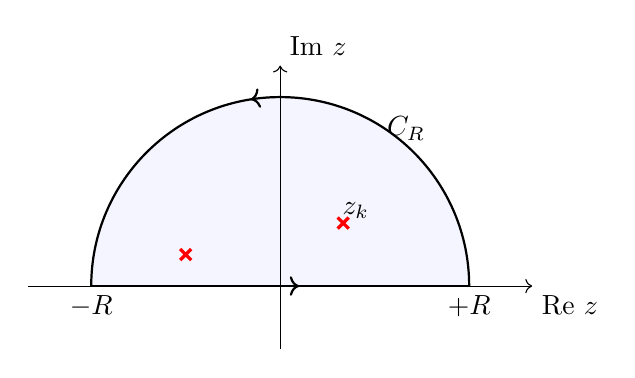
\begin{tikzpicture}[scale=0.8]
    \fill[region] (-3,0) arc (180:0:3) -- cycle;
    \draw[->] (-4,0) -- (4,0) node[below right] {Re $z$};
    \draw[->] (0,-1) -- (0,3.5) node[above right] {Im $z$};
    \draw[contour] (3,0) arc (0:180:3);
    \draw[contour] (-3,0) -- (3,0);
    \node at (3,0) [below] {$+R$};
    \node at (-3,0) [below] {$-R$};
    \node at (2,2.5) {$C_R$};
    \node[pole] at (1,1) {};
    \node[pole] at (-1.5, 0.5) {};
    \node at (1.2,1.2) {$z_k$};
\end{tikzpicture}
\end{center}

The closed loop integral is split into two parts:
\[
\oint_{\Gamma_R} = \int_{-R}^{+R} dx + \int_{C_R} dz
\]
If $\lim_{R\to\infty} \int_{C_R} R(z) dz \to 0$, then:
\[
\int_{-\infty}^{\infty} R(x) \, dx = 2\pi i \sum_{\operatorname{Im}(z_n) > 0} \res [R(z)]_{z=z_n}
\]
This convergence typically requires that $R(z)$ decays at least as $|R(z)| \le C |z|^{-2}$ as $z \to \infty$. Indeed, if this condition holds:
\[
\left| \int_{C_R} R(z) dz \right| \le \frac{C}{R^2} \cdot \pi R \to 0 \text{ as } R \to \infty
\]
In complete analogy, one may choose to close the contour in the lower half-plane. In that case:
\[
\int_{-\infty}^{\infty} R(x) \, dx = -2\pi i \sum_{\operatorname{Im}(z_n) < 0} \res [R(z)]_{z=z_n}
\]
\end{keyconcept}

\begin{examplebox}[]
Evaluate the integral:
\[
\ds I = \int_{-\infty}^{+\infty} \frac{dx}{(x^2+a^2)^3}
\]

\textbf{Derivation:}
We consider the complex function $R(z) = \frac{1}{(z^2+a^2)^3}$. We close the contour in the upper half-plane.
\[
\oint_C \frac{dz}{(z^2+a^2)^3} = \lim_{R\to\infty} \int_{-R}^{+R} \frac{dx}{(x^2+a^2)^3} + \lim_{R\to\infty} \int_{C_R} \frac{dz}{(z^2+a^2)^3} = 2\pi i \res_{z=ia} R(z)
\]
The pole in the upper half-plane is at $z=ia$ (since $z^2+a^2 = (z-ia)(z+ia)$). It is a pole of order 3.
\[
\res_{z=ia} \left[ \frac{1}{(z^2+a^2)^3} \right] = \frac{1}{2!} \frac{d^2}{dz^2} \left[ \frac{1}{(z+ia)^3} \right]_{z=ia}
\]
Calculating the derivative:
\[
= \frac{1}{2} \left[ \frac{(-3)(-4)}{(z+ia)^5} \right]_{z=ia} = \frac{1}{2} \frac{12}{(2ia)^5} = \frac{6}{32 a^5 i^5} = \frac{3}{16 a^5 i}
\]
Thus:
\[
\int_{-\infty}^{+\infty} \frac{dx}{(x^2+a^2)^3} = 2\pi i \left( \frac{3}{16 a^5 i} \right) = \boxed{\frac{3\pi}{8a^5}}
\]
\end{examplebox}

\begin{examplebox}[Wedge Contour vs Keyhole Contour]
Evaluate the integral:
\[
\ds I = \int_0^{\infty} \frac{dx}{x^3+1}
\]

\textbf{Method 1: Wedge Contour}
Let $R(z) = \frac{1}{z^3+1}$. We use a wedge contour enclosing the sector from angle $0$ to $2\pi/3$.

\begin{center}
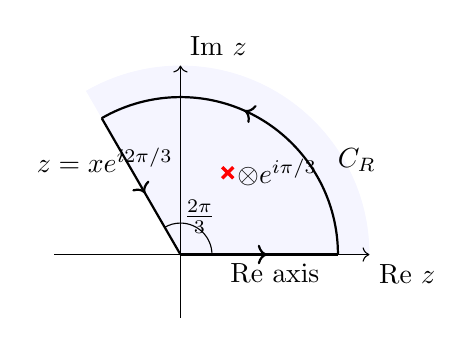
\begin{tikzpicture}[scale=0.8]
    \fill[region] (0,0) -- (3,0) arc (0:120:3) -- cycle;
    \draw[->] (-2,0) -- (3,0) node[below right] {Re $z$};
    \draw[->] (0,-1) -- (0,3) node[above right] {Im $z$};
    \draw[contour] (0,0) -- (2.5,0); % Real axis
    \draw[contour] (2.5,0) arc (0:120:2.5); % Arc
    \draw[contour] (2.5*cos{120}, 2.5*sin{120}) -- (0,0); % Return path
    \node at (1.5, -0.3) {Re axis};
    \node at (-1.2, 1.5) {$z = x e^{i 2\pi/3}$};
    \node at (2.8, 1.5) {$C_R$};
    \node[pole] at (1.5*cos{60}, 1.5*sin{60}) {};
    \node at (1.5*cos{60}, 1.5*sin{60}) [right] {$\otimes e^{i\pi/3}$};
    \draw (0.5,0) arc (0:120:0.5);
    \node at (0.3, 0.6) {$\frac{2\pi}{3}$};
\end{tikzpicture}
\end{center}

\[
\oint_C \frac{dz}{z^3+1} = \int_0^\infty \frac{dx}{x^3+1} + \int_{C_R} + \int_\infty^0 \frac{e^{2\pi i/3} dx}{(e^{2\pi i/3} x)^3 + 1} = 2\pi i \res_{z=e^{i\pi/3}} R(z)
\]
Note that $(e^{2\pi i/3})^3 = e^{2\pi i} = 1$. Thus the return path integral becomes $e^{2\pi i/3} \int_\infty^0 \frac{dx}{x^3+1}$.
\[
\left( 1 - e^{2\pi i/3} \right) \int_0^\infty \frac{dx}{x^3+1} = 2\pi i \res_{z=e^{i\pi/3}} [R(z)]
\]
The roots of $z^3+1$ are $z_1 = e^{i\pi/3}$, $z_2 = e^{i\pi}$, $z_3 = e^{-i\pi/3}$. Only $z_1$ is inside the wedge.
\[
\res_{z=e^{i\pi/3}} \left[ \frac{1}{z^3+1} \right] = \frac{1}{3z^2}\Big|_{z=e^{i\pi/3}} = \frac{1}{3 e^{2\pi i/3}}
\]
Solving for $I$:
\[
I = \frac{2\pi i}{1 - e^{2\pi i/3}} \cdot \frac{1}{3 e^{2\pi i/3}}
\]
Using identities $1 - e^{2\pi i/3} = e^{i\pi/3}(e^{-i\pi/3} - e^{i\pi/3}) = e^{i\pi/3}(-2i\sin(\pi/3))$:
\[
I = \frac{2\pi i}{-2i \sin(\pi/3) e^{i\pi/3} 3 e^{2\pi i/3}} = \frac{\pi}{3 \sin(\pi/3) e^{i\pi}} = \frac{\pi}{3 (\sqrt{3}/2) (-1)} = \boxed{\frac{2\pi}{3\sqrt{3}}}
\]

\textbf{Method 2: Keyhole Contour}
\begin{center}
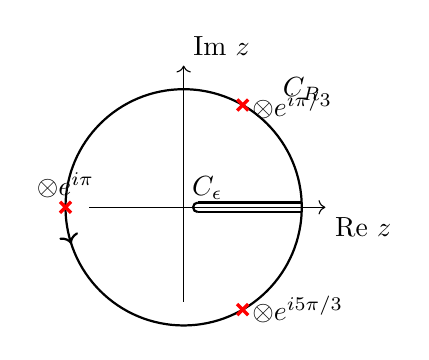
\begin{tikzpicture}[scale=0.6]
    \draw[->] (-2,0) -- (3,0) node[below right] {Re $z$};
    \draw[->] (0,-2) -- (0,3) node[above right] {Im $z$};
    % Large circle
    \draw[contour] (2.5,0) arc (0:360:2.5);
    \node at (2.5, 2.5) {$C_R$};
    % Keyhole structure
    \draw[thick] (0.3, 0.1) -- (2.5, 0.1);
    \draw[thick] (2.5, -0.1) -- (0.3, -0.1);
    % Use 'thick' instead of 'contour' for the small arc to avoid error
    \draw[thick] (0.3, 0.1) arc (90:270:0.1);
    \node at (0.5, 0.4) {$C_\epsilon$};
    
    % Poles
    \node[pole] at (1.25, 2.165) {}; 
    \node at (1.25, 2.165) [right] {$\otimes e^{i\pi/3}$};
    \node[pole] at (-2.5, 0) {}; 
    \node at (-2.5, 0) [above] {$\otimes e^{i\pi}$};
    \node[pole] at (1.25, -2.165) {}; 
    \node at (1.25, -2.165) [right] {$\otimes e^{i5\pi/3}$};
\end{tikzpicture}
\end{center}
The limits on $C_R$ and $C_\epsilon$ vanish. On the branch cut:
\[
\int_0^\infty \frac{\ln x dx}{x^3+1} + \int_\infty^0 \frac{(\ln x + 2\pi i) dx}{x^3+1} = 2\pi i \sum \res
\]
This reduces to:
\[
-2\pi i \int_0^\infty \frac{dx}{x^3+1} = 2\pi i \sum \res \left( \frac{\ln z}{z^3+1} \right)
\]
Calculating the residues at all three poles $z_{1,2,3}$ and summing them yields the same result: $\boxed{\frac{2\pi}{3\sqrt{3}}}$.
\end{examplebox}

% ==========================================
% SECTION 3: Type-III Integrals
% ==========================================
\section{Type-III Integrals}

\begin{keyconcept}[Fourier Integrals]
We consider integrals of the form:
\[
I = \int_{-\infty}^{\infty} e^{iax} R(x) \, dx
\]
Assume $a > 0$ and that for $z \in C_R$, $\max |R(z)| = M(R) \to 0$ as $R \to \infty$.
According to \textbf{Jordan's Lemma}:
\[
\lim_{R\to\infty} \int_{C_R} R(z) e^{iaz} \, dz = 0
\]

\begin{center}
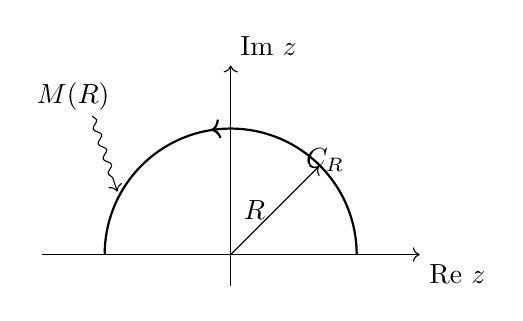
\begin{tikzpicture}[scale=0.8]
    \draw[->] (-3,0) -- (3,0) node[below right] {Re $z$};
    \draw[->] (0,-0.5) -- (0,3) node[above right] {Im $z$};
    \draw[contour] (2,0) arc (0:180:2);
    \node at (1.5, 1.5) {$C_R$};
    \draw[->] (0,0) -- (1.4, 1.4) node[midway, left] {$R$};
    \node at (-2.5, 2.5) {$M(R)$};
    \draw[->, decorate, decoration={snake, amplitude=.4mm, segment length=2mm, post length=1mm}] (-2.2, 2.2) -- (-1.8, 1.0);
\end{tikzpicture}
\end{center}

In order to estimate the contribution from the integral over $C_R$, notice that:
$|e^{iaz}| = |e^{ia(R\cos\varphi + i R\sin\varphi)}| = e^{-aR\sin\varphi}$. Since $a > 0$, the exponential decays in the upper half-plane.

Assuming $R(z)$ has no poles on the real axis:
\[
\int_{-\infty}^{+\infty} e^{iax} R(x) \, dx = 2\pi i \sum_{\operatorname{Im} z_k > 0} \res [e^{iaz} R(z)]_{z=z_k}
\]
\textbf{Notes:}
1. If $a < 0$, close the contour in the lower half-plane.
2. If $R(z)$ is real for $z=x$ and $a>0$, we can separate real and imaginary parts:
\begin{align*}
\int_{-\infty}^{+\infty} R(x) \cos(ax) \, dx &= -2\pi \operatorname{Im} \left\{ \sum_{\operatorname{Im} z_k > 0} \res [e^{iaz} R(z)] \right\} \\
\int_{-\infty}^{+\infty} R(x) \sin(ax) \, dx &= 2\pi \operatorname{Re} \left\{ \sum_{\operatorname{Im} z_k > 0} \res [e^{iaz} R(z)] \right\}
\end{align*}
\end{keyconcept}

\begin{examplebox}[]
Evaluate the integral:
\[
\ds I = \int_{-\infty}^{+\infty} \frac{(x-1) \cos(5x)}{x^2-2x+5} \, dx
\]

\textbf{Derivation:}
Consider the complex integral $I_{complex} = \oint_C \frac{(z-1)e^{i5z}}{z^2-2z+5} \, dz$.
The poles are found at $z^2-2z+5=0$, which gives $z = 1 \pm 2i$.
Only $z_1 = 1+2i$ lies in the upper half-plane ($\operatorname{Im} z_1 > 0$).
\[
\res_{z=1+2i} \left[ \frac{e^{i5z}(z-1)}{(z-z_1)(z-z_2)} \right] = \frac{(z_1-1)e^{i5z_1}}{z_1-z_2}
\]
Substitute $z_1 = 1+2i$ and $z_2 = 1-2i$:
\[
\res = \frac{(2i) e^{5i(1+2i)}}{4i} = \frac{1}{2} e^{5i - 10} = \frac{e^{-10}}{2} (\cos 5 + i \sin 5)
\]
Using the formula for the cosine integral (Real part of $e^{i5z}$, but note the $-2\pi \operatorname{Im}$ formula above derived from residue theorem logic):
\[
I = -2\pi \operatorname{Im} (\text{Residue}) = -2\pi \left( \frac{e^{-10}}{2} \sin 5 \right) = \boxed{-\pi e^{-10} \sin 5}
\]
\end{examplebox}

\begin{examplebox}[Indented Contour]
Evaluate the integral:
\[
\ds I = \int_0^{\infty} \frac{\sin x}{x} \, dx
\]

\textbf{Derivation:}
Use $f(z) = \frac{e^{iz}}{z}$. The pole at $z=0$ lies on the real axis, so we must indent the contour around it.

\begin{center}
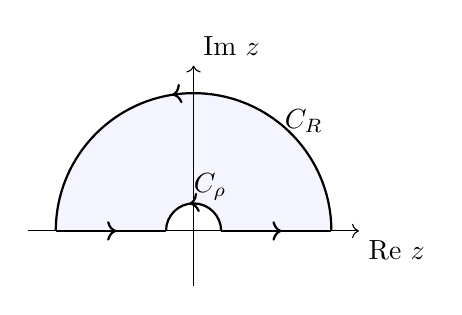
\begin{tikzpicture}[scale=0.7]
    \fill[region] (-2.5,0) -- (-0.5,0) arc (180:0:0.5) -- (2.5,0) arc (0:180:2.5) -- cycle;
    \draw[->] (-3,0) -- (3,0) node[below right] {Re $z$};
    \draw[->] (0,-1) -- (0,3) node[above right] {Im $z$};
    \draw[contour] (2.5,0) arc (0:180:2.5);
    \draw[contour] (-2.5,0) -- (-0.5,0);
    \draw[contour] (0.5,0) -- (2.5,0);
    \draw[contour] (0.5,0) arc (0:180:0.5); % Small semicircle
    \node at (2, 2) {$C_R$};
    \node at (0.3, 0.8) {$C_\rho$};
\end{tikzpicture}
\end{center}
\[
\oint_C \frac{e^{iz}}{z} dz = \lim_{R\to\infty \atop \rho\to 0} \left[ \int_{-R}^{-\rho} \frac{e^{ix} dx}{x} + \int_\rho^R \frac{e^{ix} dx}{x} + \int_{C_R} + \int_{C_\rho} \right] = 0
\]
The sum of the integrals on the real axis becomes $2i \int_0^\infty \frac{\sin x}{x} dx$.
For the small semi-circle $C_\rho$, let $z = \rho e^{i\varphi}$:
\[
\int_{C_\rho} \frac{e^{iz} dz}{z} = \lim_{\rho \to 0} \int_\pi^0 \frac{e^{i\rho e^{i\varphi}} i\rho e^{i\varphi} d\varphi}{\rho e^{i\varphi}} = \int_\pi^0 i d\varphi = -i\pi
\]
Thus:
\[
2i I - i\pi = 0 \implies \boxed{I = \frac{\pi}{2}}
\]
\end{examplebox}

\begin{examplebox}[]
Evaluate the integral:
\[
\ds I = \int_0^\infty \frac{\cos(ax) - \cos(bx)}{x^2} \, dx \quad (a \ge 0, b \ge 0)
\]

\textbf{Derivation:}
We consider the integral $\oint_C \frac{e^{iaz} - e^{ibz}}{z^2} \, dz$ over the indented contour.
Along the small semicircle $C_p$ around $z=0$:
\[
\lim_{p \to 0} \int_{C_p} \frac{e^{iaz} - e^{ibz}}{z^2} dz = \lim_{p \to 0} \int_{\pi}^{0} \frac{(1 + iap e^{i\varphi}) - (1 + ibp e^{i\varphi})}{p^2 e^{2i\varphi}} i p e^{i\varphi} d\varphi
\]
\[
= \lim_{p \to 0} \int_{\pi}^{0} \frac{i(a-b)p e^{i\varphi}}{p^2 e^{2i\varphi}} i p e^{i\varphi} d\varphi = \int_\pi^0 -(a-b) d\varphi = \pi(a-b)
\]
The integral over the real axis gives $2I$.
\[
2I + \pi(a-b) = 0 \implies \boxed{I = \frac{\pi}{2}(b-a)}
\]
\end{examplebox}

\begin{examplebox}[Rectangular Contour]
Evaluate the integral:
\[
\ds I = \int_{-\infty}^{+\infty} \frac{e^{ax}}{e^x + 1} \, dx \quad (0 < a < 1)
\]

\textbf{Derivation:}
Use a rectangular contour with height $2\pi i$.

\begin{center}
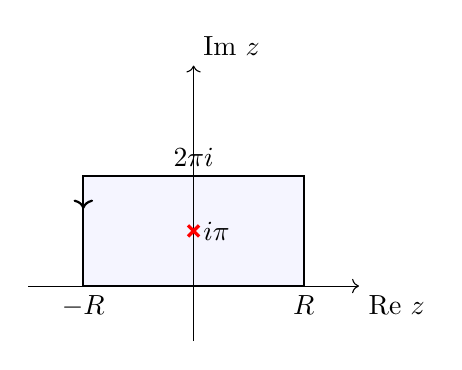
\begin{tikzpicture}[scale=0.7]
    \fill[region] (-2,0) rectangle (2,2);
    \draw[->] (-3,0) -- (3,0) node[below right] {Re $z$};
    \draw[->] (0,-1) -- (0,4) node[above right] {Im $z$};
    \draw[contour] (2,0) -- (2,2) -- (-2,2) -- (-2,0) -- cycle;
    \node at (2,0) [below] {$R$};
    \node at (-2,0) [below] {$-R$};
    \node at (0, 2) [above] {$2\pi i$};
    \node[pole] at (0, 1) {}; \node[right] at (0,1) {$i\pi$};
\end{tikzpicture}
\end{center}
The integral over the top path (from $R+2\pi i$ to $-R+2\pi i$) is:
\[
\int_R^{-R} \frac{e^{a(x+2\pi i)}}{e^{x+2\pi i} + 1} dx = -e^{2\pi i a} \int_{-R}^R \frac{e^{ax}}{e^x+1} dx
\]
The vertical segments vanish as $R \to \infty$ (provided $0 < a < 1$).
The pole at $z=i\pi$ gives a residue of:
\[
\res_{z=i\pi} \left[ \frac{e^{az}}{e^z + 1} \right] = \frac{e^{ia\pi}}{e^{i\pi}} = -e^{ia\pi}
\]
Thus:
\[
(1 - e^{2\pi i a}) I = 2\pi i (-e^{ia\pi})
\]
\[
I = \frac{-2\pi i e^{ia\pi}}{1 - e^{2\pi i a}} = \frac{2\pi i}{e^{i\pi a} - e^{-i\pi a}} = \boxed{\frac{\pi}{\sin(\pi a)}}
\]
\end{examplebox}

\begin{examplebox}[Gaussian Integral]
Evaluate the integral:
\[
\ds I = \int_0^\infty e^{-ax^2} \cos(bx) \, dx \quad (a > 0)
\]

\textbf{Derivation:}
Integrate $e^{-az^2}$ around a rectangle with height $ib/2a$. There are no poles inside.
\[
\int_I + \int_{II} + \int_{III} + \int_{IV} = 0
\]
\begin{itemize}
    \item $\int_I = \int_{-\infty}^\infty e^{-ax^2} dx = \sqrt{\frac{\pi}{a}}$.
    \item $\int_{III} = -\int_{-\infty}^\infty e^{-a(x + i\frac{b}{2a})^2} dx = -e^{b^2/4a} \int_{-\infty}^\infty e^{-ax^2} e^{-ibx} dx$.
    \item The vertical segments II and IV vanish as $R \to \infty$.
\end{itemize}
\[
\sqrt{\frac{\pi}{a}} - e^{b^2/4a} \int_{-\infty}^\infty e^{-ax^2} \cos(bx) dx = 0
\]
(The imaginary part $\sin(bx)$ vanishes due to symmetry).
\[
\boxed{I = \frac{1}{2} \sqrt{\frac{\pi}{a}} e^{-b^2/4a}}
\]
\end{examplebox}

\begin{examplebox}[]
Evaluate the integral:
\[
\ds I = \int_0^\infty e^{-\pi x} \frac{\sin(ax)}{\sinh(\pi x)} \, dx
\]

\textbf{Derivation:}
Integrate $f(z) = \frac{e^{iaz}}{e^{2\pi z} - 1}$ around a rectangle with height $1$ (indenting at poles $z=0$ and $z=i$).
Note that $f(x+i) = \frac{e^{ia(x+i)}}{e^{2\pi(x+i)} - 1} = e^{-a} f(x)$.
This leads to the relation:
\[
\oint_C = (1-e^{-a}) \int_\rho^R \frac{e^{iax} dx}{e^{2\pi x} - 1} - i \int_\rho^{1-\rho} \frac{e^{-ay} dy}{e^{2\pi i y} - 1} + \int_{C_{\rho_1}} + \int_{C_{\rho_2}} = 0
\]
By calculating the limits of the indentations at $z=0$ and $z=i$ and taking the imaginary part of the equation, we find:
\[
\boxed{I = \frac{1}{2} \frac{1+e^{-a}}{1-e^{-a}} - \frac{1}{a}}
\]
\end{examplebox}

\begin{examplebox}[Fresnel Integrals]
Evaluate the integral:
\[
\ds I_1 = \int_0^\infty \cos(x^2) \, dx, \quad I_2 = \int_0^\infty \sin(x^2) \, dx
\]

\textbf{Derivation:}
Consider $\oint_{C_R} e^{iz^2} dz$ over a sector of angle $\pi/4$.

\begin{center}
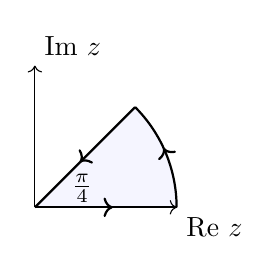
\begin{tikzpicture}[scale=0.6]
    \fill[region] (0,0) -- (3,0) arc (0:45:3) -- cycle;
    \draw[->] (0,0) -- (3,0) node[below right] {Re $z$};
    \draw[->] (0,0) -- (0,3) node[above right] {Im $z$};
    \draw[contour] (0,0) -- (3,0);
    \draw[contour] (3,0) arc (0:45:3);
    \draw[contour] (3*cos{45}, 3*sin{45}) -- (0,0);
    \node at (1, 0.4) {$\frac{\pi}{4}$};
\end{tikzpicture}
\end{center}
The integral along the return path (line at $\pi/4$) involves $z = r e^{i\pi/4}$, so $z^2 = r^2 e^{i\pi/2} = i r^2$.
\[
\int_{III} = \int_R^0 e^{i(ir^2)} e^{i\pi/4} dr = -e^{i\pi/4} \int_0^R e^{-r^2} dr = -e^{i\pi/4} \frac{\sqrt{\pi}}{2}
\]
Thus $\int_0^\infty e^{ix^2} dx = e^{i\pi/4} \frac{\sqrt{\pi}}{2} = \left( \frac{1}{\sqrt{2}} + \frac{i}{\sqrt{2}} \right) \frac{\sqrt{\pi}}{2}$.
Equating real and imaginary parts:
\[
\boxed{\int_0^\infty \cos(x^2) \, dx = \int_0^\infty \sin(x^2) \, dx = \frac{1}{2} \sqrt{\frac{\pi}{2}}}
\]
\end{examplebox}

% ==========================================
% SECTION 4: Type-IV Integrals
% ==========================================
\section{Type-IV Integrals (Mellin Transform)}

\begin{keyconcept}[Branch Cuts]
We consider integrals of the form:
\[
I = \int_0^\infty x^{\alpha-1} R(x) \, dx
\]
where $\alpha$ is a \underline{non-integer} number.
Define $h(z) = z^{\alpha-1}$ with a branch cut along the positive real axis.
\[
\begin{cases}
h(x+i0) = x^{\alpha-1} \\
h(x-i0) = x^{\alpha-1} e^{2\pi i (\alpha-1)} = e^{2\pi i \alpha} h(x)
\end{cases}
\]

\begin{center}
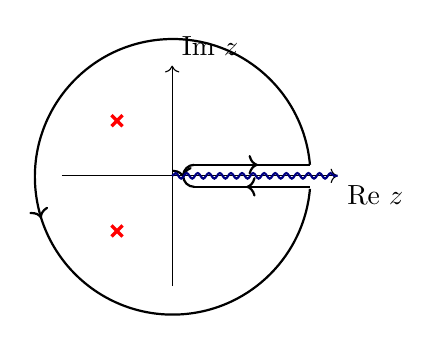
\begin{tikzpicture}[scale=0.7]
    \draw[->] (-2,0) -- (3,0) node[below right] {Re $z$};
    \draw[->] (0,-2) -- (0,2) node[above right] {Im $z$};
    \draw[contour] (2.5, 0.2) arc (5:355:2.5); % Large circle
    \draw[contour] (0.4, 0.2) arc (90:270:0.2); % Small circle
    \draw[contour] (2.5, -0.2) -- (0.4, -0.2);
    \draw[contour] (0.4, 0.2) -- (2.5, 0.2);
    \draw[branchcut] (0,0) -- (3,0);
    \node[pole] at (-1, 1) {}; \node[pole] at (-1, -1) {};
\end{tikzpicture}
\end{center}

The integral over the "upper" and "lower" banks of the cut gives $I - e^{2\pi i \alpha} I$.
\[
I (1 - e^{2\pi i \alpha}) = 2\pi i \sum_{z=z_k} \res [z^{\alpha-1} R(z)]
\]
\[
\implies I = \frac{2\pi i}{1 - e^{2\pi i \alpha}} \sum_{z=z_k} \res [z^{\alpha-1} R(z)]
\]
\end{keyconcept}

\begin{examplebox}[]
Evaluate the integral:
\[
\ds I = \int_0^\infty \frac{x^{\alpha-1}}{x+1} \, dx \quad (0 < \alpha < 1)
\]

\textbf{Derivation:}
The only pole is at $z=-1 = e^{i\pi}$.
\[
\res_{z=-1} \left[ \frac{z^{\alpha-1}}{z+1} \right] = (-1)^{\alpha-1} = (e^{i\pi})^{\alpha-1} = e^{i\pi\alpha} e^{-i\pi} = -e^{i\pi\alpha}
\]
Substituting into the formula:
\[
I = \frac{2\pi i}{1 - e^{2\pi i \alpha}} (-e^{i\pi\alpha}) = \frac{-2\pi i e^{i\pi\alpha}}{e^{i\pi\alpha}(e^{-i\pi\alpha} - e^{i\pi\alpha})} = \frac{2\pi i}{e^{i\pi\alpha} - e^{-i\pi\alpha}} = \boxed{\frac{\pi}{\sin(\pi \alpha)}}
\]
\end{examplebox}

\begin{examplebox}[]
Evaluate the integral:
\[
\ds I = \int_0^\infty \frac{x^{\alpha-1}}{(1+x^2)^2} \, dx \quad (0 < \alpha < 4)
\]

\textbf{Derivation:}
Poles at $z = \pm i$.
\[
\res_{z=i} = \frac{\alpha-2}{4} e^{i \pi \alpha / 2}, \quad \res_{z=-i} = \frac{\alpha-2}{4} e^{3i\pi \alpha / 2}
\]
Summing residues and simplifying the algebraic expression:
\[
I = \frac{2\pi i}{1 - e^{2\pi i \alpha}} \frac{\alpha-2}{4} \left( e^{i\frac{\pi\alpha}{2}} + e^{3i\frac{\pi\alpha}{2}} \right)
\]
\[
I = \boxed{\frac{\pi(2-\alpha)}{4 \sin(\pi \alpha/2)}}
\]
\end{examplebox}

\begin{examplebox}[Principal Value]
Evaluate the integral:
\[
\ds I = \int_0^\infty \frac{x^{\alpha-1}}{1-x} \, dx \quad (0 < \alpha < 1)
\]

\textbf{Derivation:}
This is a Principal Value integral due to the singularity at $x=1$. The contour must indent around $x=1$ on both the upper and lower paths of the branch cut.
The contribution from the small semi-circles at $z=1$ gives residues of $i\pi$ and $i\pi e^{2\pi i \alpha}$.
\[
(1 - e^{2\pi i \alpha}) I + i\pi (1 + e^{2\pi i \alpha}) = 0
\]
\[
I = -i\pi \frac{1 + e^{2\pi i \alpha}}{1 - e^{2\pi i \alpha}} = \boxed{\pi \cot(\pi \alpha)}
\]
\end{examplebox}

% ==========================================
% SECTION 5: Type-V Integrals
% ==========================================
\section{Type-V Integrals (Beta Function)}

\begin{keyconcept}[Integrals on Finite Intervals]
We consider integrals of the form:
\[
I = \int_0^1 \left(\frac{x}{1-x}\right)^\alpha R(x) \, dx
\]
We use a "Dog-bone" or "Dumbbell" contour wrapping around the segment $[0,1]$.

\begin{center}
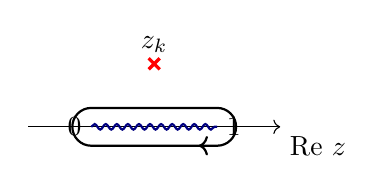
\begin{tikzpicture}[scale=0.8]
    \draw[->] (-1,0) -- (3,0) node[below right] {Re $z$};
    \draw[branchcut] (0,0) -- (2,0);
    \draw[contour] (0,0.3) -- (2,0.3) arc (90:-90:0.3) -- (0,-0.3) arc (270:90:0.3);
    \node at (0,0) [left] {0}; \node at (2,0) [right] {1};
    \node[pole] at (1,1) {};
    \node at (1,1.3) {$z_k$};
\end{tikzpicture}
\end{center}

The residue at infinity must be included.
\[
I = \frac{2\pi i}{1 - e^{2\pi i \alpha}} \left( \sum \res_{z_n} f(z) + \res_{z=\infty} f(z) \right)
\]
The residue at infinity is calculated via Laurent expansion:
\[
\res f(\infty) = -e^{i\pi\alpha} (\alpha c_0 + c_{-1})
\]
\end{keyconcept}

\begin{examplebox}[]
Evaluate the integral:
\[
\ds I = \int_0^1 \left( \frac{x}{1-x} \right)^\alpha \frac{dx}{x+1}
\]

\textbf{Derivation:}
$f(z) = \left( \frac{z}{1-z} \right)^\alpha \frac{1}{z+1}$.
\begin{itemize}
    \item Residue at $z=-1$:
    $\res_{z=-1} = 2^{-\alpha} e^{i\pi\alpha}$.
    \item Residue at $z=\infty$:
    $\res_{z=\infty} = -e^{i\pi\alpha}$.
\end{itemize}
Substituting into the formula:
\[
I = \frac{2\pi i}{1 - e^{2\pi i \alpha}} (2^{-\alpha} e^{i\pi\alpha} - e^{i\pi\alpha}) = \boxed{\frac{\pi (1-2^{-\alpha})}{\sin(\pi\alpha)}}
\]
\end{examplebox}

\begin{examplebox}[]
Evaluate the integral:
\[
\ds I = \int_0^1 \sqrt{\frac{1-x}{x}} \frac{dx}{(x+2)^2}
\]

\textbf{Derivation:}
Here $\alpha = -1/2$. $R(z) \sim 1/z^2$, so the residue at infinity is 0.
We calculate the residue at $z=-2$:
\[
\res_{z=-2} f(z) = i\pi \frac{d}{dz} [h(z)]_{z=-2} = -\frac{1}{8 h(-2)}
\]
This yields:
\[
I = \boxed{\frac{\pi}{4\sqrt{6}}}
\]
\end{examplebox}

\begin{examplebox}[]
Evaluate the integral:
\[
\ds I = \int_{-1}^{+1} \frac{\sqrt[4]{(1-x)(1+x)^3}}{1+x^2} \, dx
\]

\textbf{Derivation:}
The branch cut is $[-1, 1]$. The phases relate via $f(\tilde{x}) = -i f(x)$.
We calculate residues at $\pm i$ and $\infty$.
\[
\res_{z=i} f(z) = \frac{\sqrt{2} e^{i\pi/8}}{2i}, \quad \res_{z=-i} f(z) = -\frac{i}{\sqrt{2}} e^{3i\pi/8}
\]
\[
\res_{z=\infty} f(z) = - e^{-i\pi/4}
\]
Combining all terms:
\[
I = \boxed{\sqrt{2}\pi \left[ \sqrt{2} \cos\left(\frac{\pi}{8}\right) - 1 \right]}
\]
\end{examplebox}

% ==========================================
% SECTION 6: Type-VI Integrals
% ==========================================
\section{Type-VI Integrals (Logarithms)}

\begin{keyconcept}[Powers of Logarithms]
We consider integrals of the form:
\[
I = \int_0^\infty x^{\alpha-1} (\ln x)^m R(x) \, dx
\]
This can be solved by differentiating Type-IV integrals with respect to $\alpha$:
\[
\frac{d^m}{d\alpha^m} \int_0^\infty x^{\alpha-1} R(x) \, dx = \int_0^\infty x^{\alpha-1} \ln^m x R(x) \, dx
\]
Alternatively, integrate $f(z) = z^{\alpha-1} (\ln z)^m R(z)$ around the keyhole contour, accounting for the branch jump of logarithm: $\ln(x e^{2\pi i}) = \ln x + 2\pi i$.
\end{keyconcept}

\begin{examplebox}[]
Evaluate the integral:
\[
\ds I = \int_0^\infty \frac{\ln x \, dx}{\sqrt{x} (x+1)^2} \quad (\alpha = 1/2)
\]

\textbf{Derivation:}
Using the keyhole contour integration formula for $\alpha=1/2$ ($e^{2\pi i \alpha} = -1$):
\[
(1 - (-1)) I - 2\pi i (-1) \int_0^\infty \frac{dx}{\sqrt{x}(x+1)^2} = 2\pi i \res_{z=-1} \left[ \frac{\ln z}{\sqrt{z}(z+1)^2} \right]
\]
\[
2I + 2\pi i \int_0^\infty \frac{dx}{\sqrt{x}(x+1)^2} = 2\pi i \res_{z=-1}
\]
Calculating the residue at $z=-1$:
\[
\res_{z=-1} = \frac{d}{dz} \left( \frac{\ln z}{\sqrt{z}} \right) \bigg|_{z=-1} = \left[ \frac{1}{z\sqrt{z}} - \frac{1}{2} \frac{\ln z}{z^{3/2}} \right]_{z=-1}
\]
Using $\ln(-1) = i\pi$ and $\sqrt{-1} = i$:
\[
= \left[ -\frac{1}{i} - \frac{1}{2} \frac{i\pi}{-i} \right] = i + \frac{\pi}{2}
\]
The integral $\int_0^\infty \frac{dx}{\sqrt{x}(x+1)^2} = \frac{\pi}{2}$ (standard Type IV result).
\[
2I + 2\pi i (\pi/2) = 2\pi i (i + \pi/2) \implies 2I = -2\pi \implies \boxed{I = -\pi}
\]
\end{examplebox}

\begin{examplebox}[]
Evaluate the integral:
\[
\ds I = \int_0^\infty \frac{\ln x \, dx}{x^2+a^2}
\]

\textbf{Derivation:}
Using $\oint \frac{(\ln z)^2}{z^2+a^2} dz$ or specific branch cuts, the result is:
\[
\boxed{I = \frac{\pi}{2a} \ln a}
\]
\end{examplebox}

% ==========================================
% SECTION 7: Summation of Series
% ==========================================
\section{Summation of Series}

\begin{keyconcept}[Residue Summation Formulas]
Let $f(z)$ be a function with isolated poles (none at integers).
\begin{align*}
\sum_{n=-\infty}^{+\infty} f(n) &= -\pi \sum_{k \ge 1} \res_{z=a_k} [f(z) \cot(\pi z)] \\
\sum_{n=-\infty}^{+\infty} (-1)^n f(n) &= -\pi \sum_{k \ge 1} \res_{z=a_k} \left[ \frac{f(z)}{\sin(\pi z)} \right]
\end{align*}
\end{keyconcept}

\begin{examplebox}[]
Evaluate the series:
\[
\ds S = \sum_{n=-\infty}^{+\infty} \frac{1}{(n+a)^2}
\]

\textbf{Derivation:}
Consider $f(z) = \frac{1}{(z+a)^2}$. The pole is at $z = -a$ (order 2).
\[
S = -\pi \res_{z=-a} \left[ \frac{\cot(\pi z)}{(z+a)^2} \right]
\]
\[
\res = \frac{d}{dz} [\cot(\pi z)]_{z=-a} = \left[ -\csc^2(\pi z) \cdot \pi \right]_{z=-a} = -\frac{\pi}{\sin^2(-\pi a)}
\]
\[
S = -\pi \left( -\frac{\pi}{\sin^2(\pi a)} \right) = \boxed{\frac{\pi^2}{\sin^2(\pi a)}}
\]
\end{examplebox}

% ==========================================
% SUMMARY TABLE
% ==========================================
\newpage
\section{Summary of Contour Methods}

\begin{center}
\renewcommand{\arraystretch}{1.5}
\begin{tabular}{>{\bfseries}l l l}
\toprule
Type & Integrand Structure & Required Contour \\
\midrule
I & $R(\cos\theta, \sin\theta)$ over $[0, 2\pi]$ & Unit Circle $|z|=1$ \\
\midrule
II & Rational $R(x)$ over $(-\infty, \infty)$ & Semi-circle in UHP \\
 & $R(x)$ has pole on axis & Indented Semi-circle \\
\midrule
III & $e^{iax} R(x)$ (Fourier) & Semi-circle (Jordan's Lemma) \\
 & $e^{ax}/(e^x+1)$ & Rectangle height $2\pi$ \\
 & Gaussian $e^{-ax^2}$ & Rectangle height specific to $b$ \\
\midrule
IV & $x^{\alpha-1} R(x)$ (Mellin) & Keyhole around $\mathbb{R}^+$ branch cut \\
\midrule
V & $(x/(1-x))^\alpha$ & Dogbone around $[0,1]$ \\
\midrule
VI & $R(x) \ln x$ & Keyhole (use $\ln^2 z$ if needed) \\
\bottomrule
\end{tabular}
\end{center}

\end{document}